\begin{figure}[ht]
	\centering
	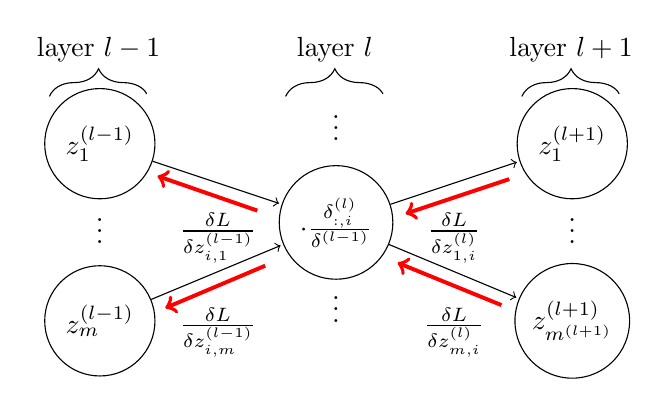
\begin{tikzpicture}[shorten >=1pt]
        \tikzstyle{unit}=[draw,shape=circle,minimum size =1.4cm]


		\draw [
            decorate,decoration={brace,amplitude=10pt},xshift=-4pt,yshift=0pt
        ] (-0.5,2.6) -- (0.75,2.6) node [black,midway,yshift=+0.6cm]{layer $l-1$};
        \node[unit](p1) at (0,2){$z_1^{(l-1)}$};
		\node at (0, 1){$\vdots$};
        \node[unit](pm) at (0,-0.25){$z_{m}^{(l-1)}$};

		\draw [
            decorate,decoration={brace,amplitude=10pt},xshift=-4pt,yshift=0pt
        ] (2.5,2.6) -- (3.75,2.6) node [black,midway,yshift=+0.6cm]{layer $l$};
		\node at (3, 2.3){$\vdots$};
        \node[unit](i) at (3,1){$\cdot\frac{\delta \z_{:,i}^{(l)}}{\delta \z^{(l-1)}}$};
		\node at (3, 0){$\vdots$};

		\draw [
            decorate,decoration={brace,amplitude=10pt},xshift=-4pt,yshift=0pt
        ] (5.5,2.6) -- (6.75,2.6) node [black,midway,yshift=+0.6cm]{layer $l+1$};
        \node[unit](k1) at (6,2){$z_1^{(l+1)}$};
		\node at (6, 1){$\vdots$};
		\node[unit](km) at (6,-0.25){$z_{m^{(l+1)}}^{(l+1)}$};

        \draw[->] (p1) -- (i);
        \draw[->] (pm) -- (i);

        \draw[->] (i) -- (k1);
		\draw[->] (i) -- (km);

        \node at (1.5,0.8){$\frac{\delta L}{\delta z_{i,1}^{(l-1)}}$};
        \node at (1.5,-0.4){$\frac{\delta L}{\delta z_{i,m}^{(l-1)}}$};

		\draw[->,red,line width=0.05cm] (2.1,0.45) -- (0.8,-0.1);
		\draw[->,red,line width=0.05cm] (2,1.15) -- (0.7,1.6);

        \node at (4.5,0.8){$\frac{\delta L}{\delta z_{1,i}^{(l)}}$};
        \node at (4.5,-0.4){$\frac{\delta L}{\delta z_{m,i}^{(l)}}$};

		\draw[->,red,line width=0.05cm] (5.1,-0.05) -- (3.75,0.5);
		\draw[->,red,line width=0.05cm] (5.2,1.55) -- (3.85,1.1);

    \end{tikzpicture}

	\caption[Backpropagation of errors through the network.]{
        Reverse traversing the network's computation graph,
        $\cdot \frac{\delta z_{:,i}^{(l)}}{\delta \w_i^{(l)}}$ is used for
        updating.\label{fig:error-backpropagation}
    }
\end{figure}
